\documentclass{article}
\usepackage{graphicx}
\usepackage{xcolor}

\title{ID2090 ASSIGNMENT: 4}
\date{}
\author{\Large Lorentz Force Equation}
\begin{document}
\maketitle
\section{CH22B104:}
\begin{flushleft}
\textbf{Name: SRINIVETHA S}

\textbf{Github id: srinivetha-24 }
\end{flushleft}
Lorentz force, the force exerted on a charged particle q moving with velocity v through an electric field E and magnetic field B. The entire electromagnetic force F on the charged particle is called the Lorentz force (after the Dutch physicist Hendrik A. Lorentz) and is given by

\textcolor{red}{\[ \vec{F} = q(\vec{E} + \vec{v} \times \vec{B}) \]}
Where:
\begin{itemize}
    \item \(q\) is the electric charge,
    \item \(\vec{E}\) is the external electric field,
    \item \(\vec{v}\) is the velocity, and
    \item \(\vec{B}\) is the magnetic field.
\end{itemize}
The first term is contributed by the electric field. The second term is the magnetic
force and has a direction perpendicular to both the velocity and the magnetic field. The
magnetic force is proportional to q and to the magnitude of the vector cross product 
\(\vec{v}\) × \(\vec{B}\). In terms of the angle \(\phi\) between  \(\vec{v}\) and
\(\vec{B}\), the magnitude of the force equals qvB \(\sin(\phi)\).
An interesting result of the Lorentz force is the motion of a charged particle in a
uniform magnetic field. If \(\vec{v}\) is perpendicular to \(\vec{B}\) (i.e., with the
angle \(\phi\) between \(\vec{v}\) and \(\vec{B}\) of 90°), the particle will follow a
circular trajectory with a radius of r = mv/qB. If the angle \(\phi\) is less than 90°,
the particle orbit will be a helix with an axis parallel to the field lines. If \(\phi\)
is zero, there will be no magnetic force on the particle, which will continue to move
undeflected along the field lines. Charged particle accelerators like cyclotrons make
use of the fact that particles move in a circular orbit when \(\vec{v}\) and \(\vec{B}\)
are at right angles. Two step transformation of lorentz force is also 
given.\cite{ref=article}\\

\begin{figure}[htp]
    \centering
    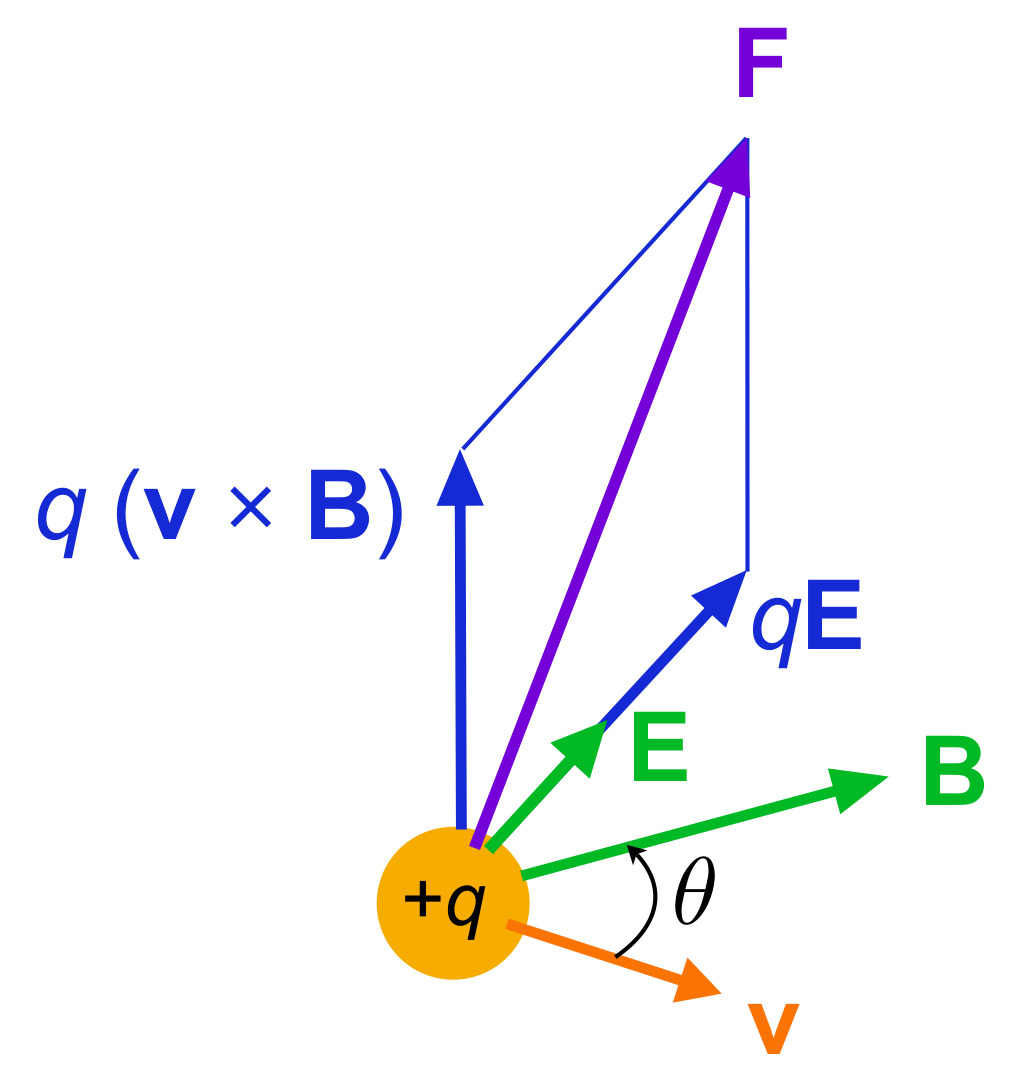
\includegraphics[width=4cm]{Lorentz_force_particle}
    \caption{Vector description of lorentz force}
    \label{fig:lorentz force vector}
\end{figure}
The magnetic force on a moving charge reveals the sign of the charge carriers in a
conductor. A current flowing from right to left in a conductor can be the result of
positive charge carriers moving from right to left or negative charges moving from left
to right, or some combination of each. When a conductor is placed in a \(\vec{B}\) field
perpendicular to the current, the magnetic force on both types of charge carriers is in
the same direction. This force gives rise to a small potential difference between the
sides of the conductor is Known as the Hall effect.\\
This force also acts on a point charge due to the electromagnetic field. Lorentz force
describes the equations of mathematical nature and the physical importance of forces
that act on charged particles. These particles can also travel through space that
contains an electric and magnetic field. Furthermore, \cite{ref=art} lorentz force is related to
Maxwell's equations.\\
I have chosen this topic primarily due to its simplicity and its relevance to my PH1020
course. The equation and concept associated with it are relatively straightforward,
making it an ideal choice for exploration and understanding.


\bibliography{citation-1}
\bibliographystyle{plain}


\end{document}
